    \section{Cinética química}\label{sec:cinetica-quimica}

    \begin{center}
        \begin{definicion}[width=0.9\textwidth]{Cinética Química}
            La \rojon{Cinética química} se encarga del estudio de la velocidad de las reacciones químicas y los factores que la afectan.
        \end{definicion}
    \end{center}

    La cinética química relaciona los mecanismos moleculares de ruptura y formación de enlaces tomando en consideración el \negrita{tiempo} a partir de magnitudes macroscópicas y microscópicas.

    \section{Velocidad de reacción}\label{sec:velocidad-de-reaccion}

    De manera general, podemos decir que la velocidad de reacción nos mide la aparición o desaparición de una sustancia con el tiempo en una reacción química.

    \begin{center}
        \begin{definicion}[width=0.9\textwidth]{Velocidad Instantánea de Reacción}
            Definimos \rojon{Velocidad instantánea} como la derivada de la concentración de una especie respecto del tiempo y podemos definir la velocidad de desaparición de los reactivos así como la velocidad de aparición de los productos.

            Su unidad, por tanto, será: \unit{\mole\per\litre\per\s} o bien \unit{\m\per\s}
        \end{definicion}
    \end{center}


    Sea una reacción general del tipo:
    \begin{equation}
        \ch{a\ A + b\ B -> c\ C + d\ D} \label{eq:general}
    \end{equation}

    Podemos definir, por tanto, tanto las velocidades de desaparición como las velocidades de aparición de la siguiente manera:
    \begin{enumerate}[label=\numberballmDarkTeal]
        \item \negsubro{Velocidades de desaparición}: tenemos que poner signo negativo para que la velocidad obtenga un signo positivo debido a que las concentraciones de los reactivos disminuyen con el tiempo.
        \begin{paracol}{2}
            \begin{equation}
                v_A = -\ \dfrac{1}{a}\ \dfrac{d[A]}{dt}\label{eq:velocidad-a}
            \end{equation}
            \switchcolumn
            \begin{equation}
                v_B = -\ \dfrac{1}{b}\ \dfrac{d[B]}{dt}\label{eq:velocidadb}
            \end{equation}
        \end{paracol}
        También lo podemos escribir como:
        \begin{paracol}{2}
            \begin{equation}
                v_A = -\ \dfrac{1}{a}\ \dfrac{\Delta[A]}{\Delta t}\label{eq:velocidad-a-incremento}
            \end{equation}
            \switchcolumn
            \begin{equation}
                v_B = -\ \dfrac{1}{b}\ \dfrac{\Delta[B]}{\Delta t}\label{eq:velicudad-b-incremento}
            \end{equation}
        \end{paracol}
        \item \negsubro{Velocidad de aparición}: se hace tomando como referencia los productos quedando por tanto sus velocidades como:
        \begin{paracol}{2}
            \begin{equation}
                v_C = +\ \dfrac{1}{c}\ \dfrac{d[C]}{dt}\label{eq:velocidad-c}
            \end{equation}
            \switchcolumn
            \begin{equation}
                v_D= +\ \dfrac{1}{d}\ \dfrac{d[D]}{dt}\label{eq:velocidadd-d}
            \end{equation}
        \end{paracol}
        o bien,
        \begin{paracol}{2}
            \begin{equation}
                v_C = +\ \dfrac{1}{c}\ \dfrac{\Delta[C]}{\Delta t}\label{eq:velocidad-c-incremento}
            \end{equation}
            \switchcolumn
            \begin{equation}
                v_D= +\ \dfrac{1}{d}\ \dfrac{\Delta [D]}{\Delta t}\label{eq:velocidad-d-incremento}
            \end{equation}
        \end{paracol}
        Las concentraciones de los productos a diferencia de los reactivos aumentan con el tiempo.
    \end{enumerate}
    A continuación, tenemos la representación de como varía la concentración de las especies con el tiempo de la reacción:

    \begin{equation*}
        \ch{H2 + I2 -> 2 HI}
    \end{equation*}

    \begin{figure}[H]
        \centering
        % [FIGURA ORIGINAL] \includegraphics[scale=.5]{images/imagesUD5CineticaQuimica/UD5_Teoria/velocidadreaccion}
        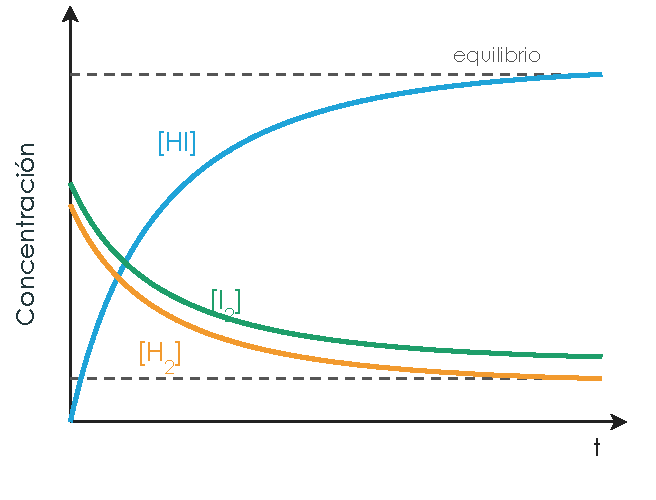
\includegraphics[width=0.55\linewidth]{FigurasSVG/UD5_Cinetica_Quimica/pdf/UD5_01_velocidad_reaccion_HI.pdf}
        \caption{Variación de las concentraciones de reactivos y productos con relación al tiempo en la reacción de hidrógeno molecular con yodo molecular}
        \label{fig:velocidadreaccion}
    \end{figure}

    Al introducir estos coeficientes estequiométricos en la velocidad conseguimos que \ul{la velocidad calculada respecto a cualquier reactivo o producto sea la misma}, es decir:
    \begin{equation}
        v = -\ \dfrac{1}{a}\ \dfrac{d[A]}{dt} =  -\ \dfrac{1}{b}\ \dfrac{d[B]}{dt} =  \dfrac{1}{c}\ \dfrac{d[C]}{dt} =   \dfrac{1}{d}\ \dfrac{d[D]}{dt}\label{eq:velocidad-todas}
    \end{equation}

    Con esto en lugar de velocidades de reacción referidas a un reactivo o un producto podemos hablar de una única velocidad de reacción.

    Por ejemplo, veamos la obtención de metanal a partir de metanol según la ecuación:
    \begin{center}
        \ch{2 CH3OH\ (g) + O2\ (g) -> 2 HCOH\ (g) + 2 H2O\ (g) }
    \end{center}
    La velocidad calculada a partir de cualquier reactivo sería:
    \begin{equation}
        v = -\ \dfrac{1}{2}\ \dfrac{d[\ch{CH3OH}]}{dt} =  -\  \dfrac{d[\ch{O2}]}{dt} =  \dfrac{1}{2}\ \dfrac{d[\ch{HCHO}]}{dt} =   \dfrac{1}{2}\ \dfrac{d[\ch{H2O}]}{dt}\label{eq:velocidad-todas-ejemplo}
    \end{equation}

    \negsubro{IMPORTANTE:} la velocidad al ser una magnitud tendrá, por tanto, su unidad.
    La concentración se suele representar en \si{\mole\per\litre}.
    Si el tiempo lo tenemos en segundos, tendremos, en consecuencia, que la unidad de la velocidad será: \si{\mole\per\litre\per\s}  o lo que es lo mismo \si{\mole\litre^{-1}\s^{-1}}


    \section{Ecuación de velocidad}\label{sec:ecuacion-de-velocidad}

    Las velocidades vistas anteriormente las podemos expresar mediante una ecuación a la que denominaremos \azuln{ecuación de velocidad} que expresa la velocidad de una reacción en un determinado instante en función de las concentraciones de las sustancias presentes en ese momento.
    Si consideramos la reacción general de la expresión \eqref{eq:general} tendríamos:
    \begin{equation}
        v = K\ [A]^\alpha\ [B]^\beta\label{eq:ecuacion-velocidad-general}
    \end{equation}

    \vspace*{-6pt}
    siendo:
    \begin{itemize}
        \item La constante $\bm{k}$ se llama \azuln{constante de velocidad}.
        Esta constante tendrá unidades y sus unidades dependerá del orden total o global de la reacción (ver más adelante)
        \item Los exponentes $\bm{\alpha}$ y $\bm{\beta}$ a los que están elevadas las concentraciones de los reactivos se llama \azuln{órdenes parciales de reacción}.
        \item A la suma de $\bm{\alpha}$ y $\bm{\beta}$ se le conoce como \azuln{orden total} o \azuln{orden global}  de la reacción.
        \item Las unidades de la constante de velocidad $\bm{k}$ dependerán, por tanto, del orden global de la reacción.
        \item Conociendo las unidades de la constante de velocidad \( \bm{k} \) podemos obtener fácilmente el orden global de la reacción.
        \item A un mayor valor de $\bm{k}$ la velocidad de reacción será mayor.
    \end{itemize}

    \negsubro{IMPORTANTE}: los coeficientes parciales de reacción no deben confundirse con los coeficientes estequiométricos ($a\ , b\ , c\ , d\ $) y se deben calcular de manera independiente.
    Si es cierto que cuando una reacción es \azuln{elemental} (más adelante se verá lo que es una reacción elemental) los órdenes parciales y los coeficientes estequiométricos coinciden.

    Como podemos de la ecuación \eqref{eq:ecuacion-velocidad-general} solo aparencen los reactivos mientras que los productos han desaparecido.
    En la ecuación de velocidad solo tendremos en cuenta la concentración de los reactivos.

    \subsection{Ecuación de velocidad de los casos más significativos}\label{sec:casos_significativos}

    Consideremos un caso muy simple en el que tenemos una reacción del tipo:
    \begin{equation*}
        \ch{A -> Productos}
    \end{equation*}
    y además, consideraremos que la reacción que se produce es elemental de modo que podemos tener que  $v = k\ [A]^\alpha $ o bien $v = - \dfrac{d[A]}{dt}$.
    Si igualamos ambas expresiones tendremos que:
    \begin{equation*}
        k\ [A]^\alpha = - \dfrac{d[A]}{dt}
    \end{equation*}
    reorganizando términos tendremos que:
    \begin{equation*}
        \dfrac{d[A]}{[A]^\alpha} = -k\  dt
    \end{equation*}
    Si integramos entre el instante $t=0$ donde tendremos una concentración de $A$ de $[A]_0$ y entre el instante $t$ donde la concentración de $A$ es de $[A]_t$ tendremos que:
    \begin{equation*}
        \int_{[A]_0}^{[A]_t} \dfrac{d[A]}{[A]^\alpha}= -k\int_{t_0}^{t} dt
    \end{equation*}

    \begin{enumerate}[label=\numberballmDarkTeal]
        \item \negsubro{Orden cero}. $\alpha = 0$.
        Tendremos que:
        \begin{equation}
        [A]
            _t = [A]_0 -K\ t\label{eq:cinetica-orden-cero}
        \end{equation}
        Si representamos $[A]$ frente el tiempo tendremos una gráfica lineal del tipo:
        \begin{figure}[H]
            \centering
            % [FIGURA ORIGINAL] \includegraphics[scale=.5]{images/imagesUD5CineticaQuimica/UD5_Teoria/ordencero}
            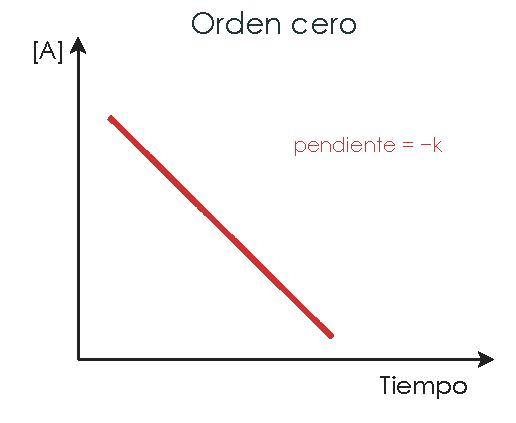
\includegraphics[width=0.45\linewidth]{FigurasSVG/UD5_Cinetica_Quimica/pdf/UD5_02_orden_cero.pdf}
            \caption{Cinética de orden cero}
            \label{fig:ordencero}
        \end{figure}
        \item \negsubro{Orden uno}. $\alpha = 1$.
        Tendremos que:
        \begin{equation}
        [A]
            _t = [A]_0\ e^{-K\ t}\label{eq:cinetica-orden-uno}
        \end{equation}
        esta ecuación la podríamos escribir como:
        \begin{equation*}
        [A]
            _t = [A]_0\ \exp\left(-K\ t\right)\label{eq:cinetica-orden-uno-integrada}
        \end{equation*}
        Si tomamos logaritmos neperianos
        \begin{equation}
            \ln [A]_t = \ln [A]_0 - K\ t\label{eq:cinetica-orden-uno-ln}
        \end{equation}
        Si representamos $\ln [A]$ frente el tiempo tendremos una gráfica lineal del tipo:
        \begin{figure}[H]
            \centering
            % [FIGURA ORIGINAL] \includegraphics[scale=.5]{images/imagesUD5CineticaQuimica/UD5_Teoria/ordenuno}
            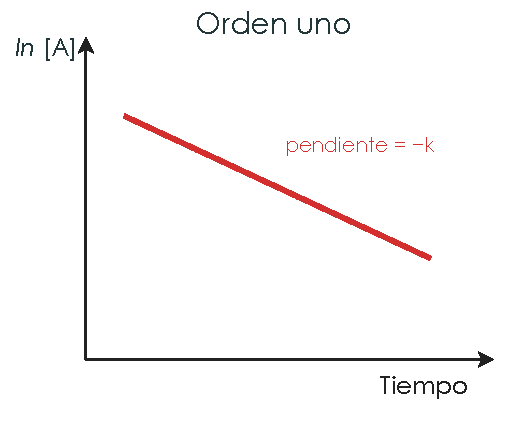
\includegraphics[width=0.45\linewidth]{FigurasSVG/UD5_Cinetica_Quimica/pdf/UD5_03_orden_uno.pdf}
            \caption{Cinética de orden uno}
            \label{fig:ordenuno}
        \end{figure}
        \item \negsubro{Orden dos}. $\alpha = 2$.
        Tendremos que:
        \begin{equation}
            \dfrac{1}{[A]_t} - \dfrac{1}{[A]_0} = k\ t\label{eq:cinetica-orden-dos}
        \end{equation}
        Reagrupando la ecuación la podemos escribir como:
        \begin{equation}
            \dfrac{1}{[A]_t}  =  \dfrac{1}{[A]_0} + k\ t  \label{eq:cinetica-orden-dos-ordenada}
        \end{equation}
%          \begin{equation}
%              [A]_t = \dfrac{[A]_0}{1 + [A]_0\ k\ t}\label{eq:cinetica-orden-dos-integrada}
%          \end{equation}
        Si representamos $\frac{1}{[A]}$ frente el tiempo tendremos una gráfica lineal del tipo:
        \begin{figure}[H]
            \centering
            % [FIGURA ORIGINAL] \includegraphics[scale=.5]{images/imagesUD5CineticaQuimica/UD5_Teoria/ordendos}
            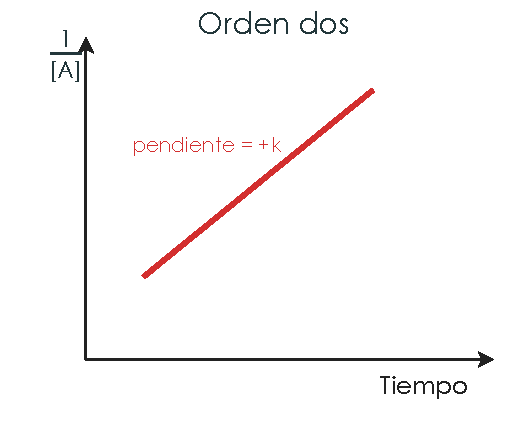
\includegraphics[width=0.45\linewidth]{FigurasSVG/UD5_Cinetica_Quimica/pdf/UD5_04_orden_dos.pdf}
            \caption{Cinética de orden dos}
            \label{fig:ordendos}
        \end{figure}
    \end{enumerate}


    \begin{enumerate}
        \item Todas las gráficas mostradas consiste en una línea recta, eso es así para obtener con facilidad los parámetros que necesitamos.
        \item Debemos fijarnos en lo que se representa en el eje \( y \) ya que en el eje \( x \) siempre tendremos el tiempo.
    \end{enumerate}

    \subsection{Cálculo de las órdenes parciales y orden global de la reacción}\label{subsec:calculo-de-las-ordenes-parciales-y-orden-global-de-la-reaccion}

    \subsubsection{Método de las velocidades iniciales}

    Es el método más utilizado y muy útil, ya que nos permite los órdenes parciales y orden global de la reacción y la constante de velocidad.
    Para su explicación veamos el siguiente ejemplo:

    Sea la reacción:
    \begin{equation*}
        \ch{CO\ (g) + NO2\ (g) -> CO2\ (g) + NO\ (g) }
    \end{equation*}
    De esta reacción nos dan los siguientes datos experimentales:
    \begin{table}[H]
        \centering
        \begin{tblr}{|c|c|c|c|}
            \hline
            \negrita{Experiencia} & $[\ch{CO}]_0$ (\si{\mole\per\litre}) & $[\ch{NO2}]_0$ (\si{\mole\per\litre}) & $v_0$ (\si{\mole\per\litre\per\s}) \\
            \hline
            1                     & \num{2e-4}                           & \num{0.5e-4}                          & \num{1.9e-8}                       \\
            \hline
            2                     & \num{2e-4}                           & \num{1.0e-4}                          & \num{3.8e-8}                       \\
            \hline
            3                     & \num{4e-4}                           & \num{0.5e-4}                          & \num{3.8e-8}                       \\
            \hline
        \end{tblr}\label{tab:table-ejemplo-orden-de-reaccion}
    \end{table}
    Primero lo que debemos hacer es poner la ecuación de la velocidad que en este caso sería:
    \begin{equation*}
        v = k\ [\ch{CO}]^\alpha \ [\ch{NO2}]^\beta
    \end{equation*}
    Como podemos ver, para escribir la ecuación de velocidad, debemos poner \(v\) y luego lo igualamos a la correspondiente constante de velocidad \(k\) y luego lo multiplicamos por la concentración de los REACTIVOS elevado a sus correspondientes coeficientes órdenes de reacción (en este caso parciales)

    Como lo que me están dando son velocidades iniciales, la expresión anterior la puedo escribir de la manera:
    \begin{equation*}
        v_0 = k\ [\ch{CO}]_0^\alpha \ [\ch{NO2}]_0^\beta
    \end{equation*}
    Como, tenemos tres experimentos, podemos tener entonces que:
    \begin{gather*}
        v_{01} = k\ [\ch{CO}]_{01}^\alpha \ [\ch{NO2}]_{01}^\beta \separ
        v_{02} = k\ [\ch{CO}]_{02}^\alpha \ [\ch{NO2}]_{02}^\beta \separ
        v_{03} = k\ [\ch{CO}]_{03}^\alpha \ [\ch{NO2}]_{03}^\beta \separ
    \end{gather*}
    Si dividimos las velocidades $v_{01}$ y $v_{02}$ podemos ver como la concentración del monóxido de carbono desaparece quedando tan solo la del dióxido de nitrógeno permitiendo así obtener $\beta$
    \begin{gather*}
        \dfrac{v_{01}}{v_{02}} = \dfrac{k\ [\ch{CO}]_{01}^\alpha \ [\ch{NO2}]_{01}^\beta}{k\ [\ch{CO}]_{02}^\alpha \ [\ch{NO2}]_{02}^\beta}\separ
        \dfrac{v_{01}}{v_{02}} = \dfrac{k\ [(\num{2e-4})^\alpha \ [(\num{1.9e-8})^\beta}{k\ [(\num{2e-4})^\alpha \ [(\num{3.8e-8})^\beta}
    \end{gather*}
    Si operamos tendremos que:
    \begin{gather*}
        \dfrac{\num{1.9e-8}}{\num{3.8e-8}} = \dfrac{k\ [\ch{CO}]_{01}^\alpha \ [\ch{NO2}]_{01}^\beta}{k\ [\ch{CO}]_{02}^\alpha \ [\ch{NO2}]_{02}^\beta}\separ
        \dfrac{\num{1.9e-8}}{\num{3.8e-8}} = \dfrac{\cancelred{k}\ \cancelred{[(\num{2e-4})^\alpha} \ [(\num{0.5e-4})^\beta}{\cancelred{k}\ \cancelred{[(\num{2e-4})^\alpha} \ [(\num{1.0e-4})^\beta}\separ
        \dfrac{1}{2} = \left( \dfrac{1}{2} \right)^\beta\separ
        0.5 = 0.5^\beta \separ
        \beta = \log_{0.5}(0.5)\separ
        \tcboxmath[opteqA]{\beta = 1}
    \end{gather*}
    Si en vuestra calculadora no podéis poner los logaritmos con la base que salga, podéis hacer un cambio de base según (siendo $c$ la nueva base):
    \begin{equation*}
        log_{b}(x) = \dfrac{log_{c}(x)}{log_{c}(b)}
    \end{equation*}
    Si ahora hacemos un tratamiento similar, pero dividiendo $v_{01}$ y $v_{03}$ obtendríamos el valor de $\alpha = 1$.
    Para obtener el valor del orden total de la reacción tendremos que sumar $\alpha$ y $\beta$ siendo en este caso $2$.

    Para obtener el valor de la constante de velocidad, solo tenemos que irnos a cualquier expresión de la velocidad y sustituir los valores de las órdenes parciales de reacción por su valor, obteniendo finalmente que $k = 1.9\ \si{\mol^{-1}\litre\s^{-1}}$ es decir $k = \SI{1.9}{\litre\per\mole\per\s}$

    \subsubsection{Método gráfico}
    Consiste en realizar representaciones gráficas según las ecuaciones vistas en el apartado \ref{sec:casos_significativos} y viendo que gráficas encajan mejor según el orden de reacción.


    \section{Reacciones directas e inversas}

    Hasta ahora hemos visto siempre la reacción directa, es decir el paso en el que los reactivos $A$ y $B$ pasan a los productos $C$ y $D$.
    Sin embargo, en ocasiones esos productos cuando se van formando, vuelven a reaccionar entre sí para dar de nuevo los reactivos de partida.
    A esta reacción entre los productos para dar de nuevo los reactivos se denomina \azuln{reacción inversa}.
    Cuando tenemos un caso así, se suele representar con una doble flecha de la siguiente manera:
    \begin{equation*}
        \ch{a\ A + b\ B <=> [reacción\ directa\ (d)][reacción\ inversa\ (i)] c\ C + d\ D} \label{eq:general_equilibrio}
    \end{equation*}
    Ambas velocidades quedarían, por tanto:
    \begin{paracol}{2}
        \begin{equation*}
            v_d = k_d\ [A]^a\ [B]^b
        \end{equation*}
        \switchcolumn
        \begin{equation*}
            v_i = k_i\ [C]^c\ [D]^d
        \end{equation*}
    \end{paracol}
    En este caso, podemos poner los coeficientes estequiométricos como órdenes parciales de reacción porque nos encontramos en una reacción elemental en cada sentido.

    Cuando las velocidades de la reacción directa se igualan con las velocidades de la reacción inversa se dice que se alcanza el \rojon{equilibrio químico} y al cociente entre ambas constantes de velocidad se le denomina \rojon{constante de equilibrio químico}
    \begin{gather*}
        v_d = v_i\separ
        k_d\ [A]^a\ [B]^b = k_i\ [C]^c\ [D]^d
    \end{gather*}
    Podemos deducir que:
    \begin{equation*}
        \dfrac{k_d}{k_i} = \dfrac{[C]^c\ [D]^d}{[A]^a\ [B]^b}
    \end{equation*}
    Por lo tanto
    \begin{equation*}
        k_{\text{equilibrio}} = \dfrac{k_d}{k_i}
    \end{equation*}
    Y también podemos decir que:
    \begin{equation}
        k_{\text{equilibrio}} = \dfrac{[C]^c\ [D]^d}{[A]^a\ [B]^b}
    \end{equation}
    \begin{figure}[H]
        \centering
        % [FIGURA ORIGINAL] \includegraphics[scale=.5]{images/imagesUD5CineticaQuimica/UD5_Teoria/equilibrio_cinetica}
        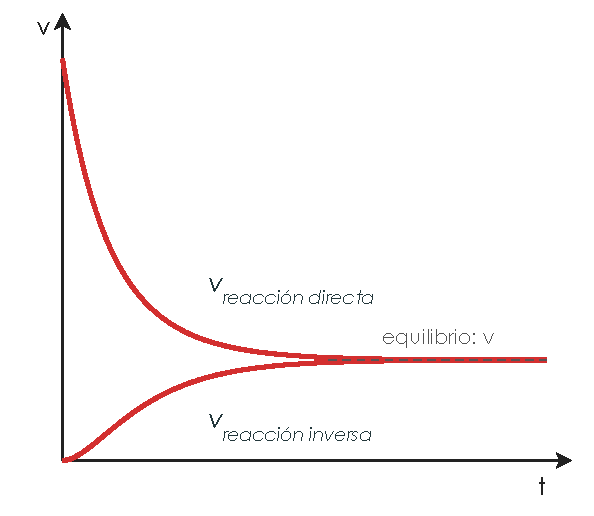
\includegraphics[width=0.5\linewidth]{FigurasSVG/UD5_Cinetica_Quimica/pdf/UD5_05_equilibrio_velocidades.pdf}
        \caption{Equilibrio químico}
        \label{fig:equilibrio_cinetica.png}
    \end{figure}


    \section{Teorías sobre las reacciones químicas}\label{sec:teorias-sobre-las-reacciones-quimicas}

    \subsection{Teoría de colisiones}\label{subsec:teoria-de-colisiones}
    Este teoría fué enunciada por Lewis en 1918 y dice:
    \caja{La \rojon{teoría de colisiones} de Lewis propone que las reacciones químicas se producen por choques entre las moléculas}
    La velocidad de reacción según esta teoría dependerá, por tanto, de los siguientes factores:
    \begin{enumerate}[label=\numberballmDarkTeal]
        \item \azuln{Frecuencia de choque por unidad de volumen}.
        A mayor número de choques, la velocidad de reacción será mayor.
        \item \azuln{Eficacia del choche}.
        Además de tener una alta frecuencia, los choques deben ser lo suficientemente efectivos para que se lleve a cabo la reacción y para ello se necesitará:
        \begin{enumerate}
            \item Los choques deben tener una energía cinética que sea suficiente para romper los enlaces necesarios.
            A esta energía suficiente se le denomina \azuln{energía de activación, $E_a$}.
            \item La fracción de moléculas que tenían esa energía o superior las calculó Ludwig Boltzmann y eran de:
            \begin{equation*}
                e^{-\frac{E_a}{R\ T}}
            \end{equation*}
            A partir de este momento, esta expresión la escribiremos como:
            \begin{equation}
                \exp\biggl(-\dfrac{E_a}{RT}\biggr)\label{eq:expresion_Boltzman}
            \end{equation}
            \item Orientación adecuada además de tener la suficiente energía.
        \end{enumerate}
    \end{enumerate}

    Teniendo en cuenta todas estas consideraciones, la \azuln{ecuación de Arrhenius} permite calcular el valor de la constante de velocidad según la expresión:
    \begin{equation}
        k = A\ e^{-\frac{E_a}{R T}}\label{eq:Arrhenius}
    \end{equation}
    La ecuación \eqref{eq:Arrhenius} a partir de ahora la escribiremos de la siguiente forma:
    \begin{equation}
        k = A\exp\biggl(-\dfrac{E_a}{RT}\biggr)\label{eq:Arrhenius_b}
    \end{equation}


    \begin{itemize}
        \item $A$: factor de frecuencia.
        \item $R$: constante de los gases ideales en julios.
        \item $T$: temperatura absoluta, es decir en kelvin.
        \item $E_a$: energía de activación.
    \end{itemize}

    \subsection{Teoría del estado de transición o complejo activado}\label{subsec:teoria-del-estado-de-transicion-o-complejo-activado}

    \negrita{H. Eyring} propuso que cuando las moléculas de los reactivos chocan, se forma una especie intermedia denominada \azuln{complejo activado} o \azuln{complejo de transición}.

    \begin{figure}[H]
        \centering
        \subfloat[Exotérmica]{
            % [FIGURA ORIGINAL] \includegraphics[scale=.45]{images/imagesUD5CineticaQuimica/UD5_Teoria/endotermica}
            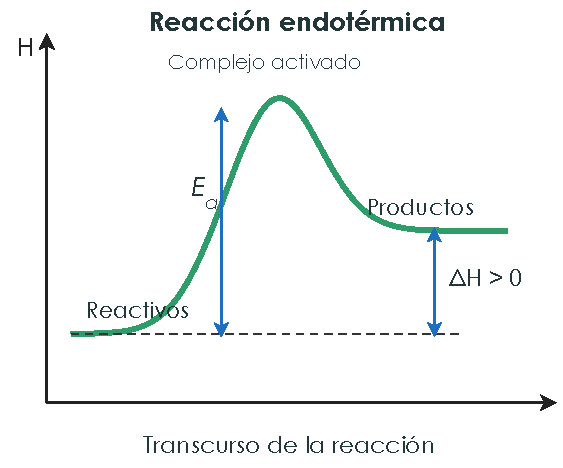
\includegraphics[width=0.31\linewidth]{FigurasSVG/UD5_Cinetica_Quimica/pdf/UD5_07_perfil_endotermica.pdf}
            \label{fig:exotermica}
        }
        \subfloat[Endotérmica]{
            % [FIGURA ORIGINAL] \includegraphics[scale=.45]{images/imagesUD5CineticaQuimica/UD5_Teoria/exotermica}
            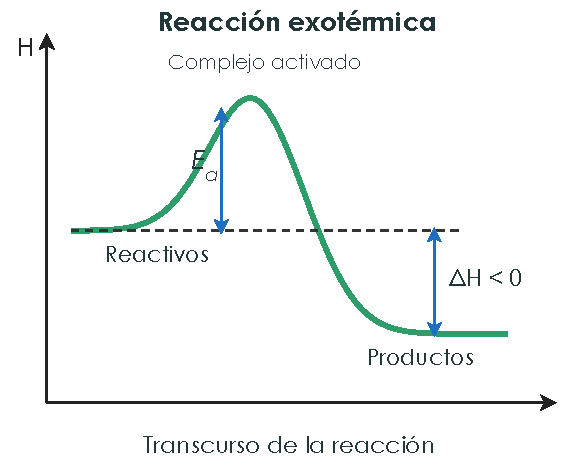
\includegraphics[width=0.31\linewidth]{FigurasSVG/UD5_Cinetica_Quimica/pdf/UD5_06_perfil_exotermica.pdf}
            \label{fig:endotermica}
        }
        \subfloat[Complejo Activado]{
            \vspace*{6pt}
            % [FIGURA ORIGINAL] \includegraphics[scale=.35]{images/imagesUD5CineticaQuimica/UD5_Teoria/complejo_activado}
            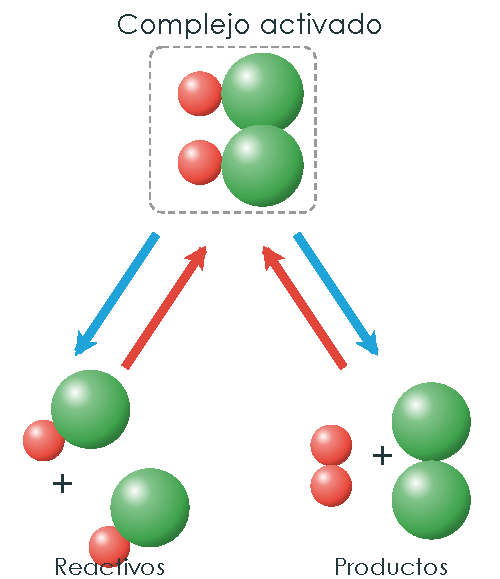
\includegraphics[width=0.25\linewidth]{FigurasSVG/UD5_Cinetica_Quimica/pdf/UD5_08_complejo_activado.pdf}
            \label{fig:complejo_activado}
        }
        \caption{}
    \end{figure}


    En la imagen, podemos ver como en este caso la energía de activación ($E_a$) es la energía que debemos suministrar para formar dicho complejo activado, así cuando menor sea la energía más fácil será que las moléculas del reactivo se dispongan para formar dicho complejo y más rápida, por tanto, será la reacción.

    Ese complejo activado es una especie de muy alta energía y de una corta duración.


    \section{Mecanismo de reacción}\label{sec:mecanismo-de-reaccion}

    Existen reacciones que se producen en una sola etapa como:
    \begin{center}
        \formula{Cl2 \gas{} + H2 \gas{} -> 2 HCl \gas{}}\\
        \formula{CH3Br \aq{} + OH- \aq{} -> CH3OH \aq{} + Br- \aq{}}
    \end{center}

    A las reacciones que se producen en una sola etapa se les denominan \rojon{reacciones elementales}

    Sin embargo, muchas reacciones químicas se llevan a cabo en varias etapas.
    A cada etapa será una \negrita{reacción elemental}.

    \subsection{Velocidad de las etapas elementales y la reacción global}\label{subsec:velocidad-de-las-etapas-elementales-y-la-reaccion-global}
    Cuando una reacción se realiza en varias etapas, su velocidad global dependerá de la velocidad de cada etapa o reacción elemental siendo, por tanto, su velocidad la combinación lineal de todas ellas.

    Si se diera el caso de que una de esas etapas fuera mucho más lenta que las demás, las velocidades de las otras reacciones se pueden desprender.
    A esta etapa o reacción que determina la velocidad de la reacción global se le denomina \negrita{etapa limitante} o \negrita{etapa controlante de la velocidad}.

    Sea por ejemplo la reacción:
    \begin{center}
        \formula{NO2 \gas{} + CO \gas{} -> NO \gas{} + CO2 \gas{}}
    \end{center}
    Esta ecuación tiene por ecuación de velocidad $v = k\ [\formula{NO2}]^2$.
    A partir de su ecuación de velocidad podemos ver que no se trata de una reacción elemental puesto que no aparece \conc{CO}.
    Las etapas propuestas para su mecanismo sería:
    \begin{gather*}
        \formula{NO2 \gas{} + NO2 \gas{} -> NO3 \gas{} + NO \gas{}};\quad v_1 = k_1\ \conc{NO2}^2\separ
        \formula{NO3 \gas{} + CO \gas{} -> NO2 \gas{} + CO2 \gas{}};\quad v_2 = k_2\ \conc{NO3}\ \conc{CO}
    \end{gather*}
    La primera etapa es mucho más lenta que la segunda y, por tanto, actúa como etapa limitante pudiéndose descartar la segunda reacción.
    Como vemos también el mecanismo de reacción, en la reacción global no aparece el \conc{NO3}, esto es debido a que es un \negrita{intermedio de reacción}, es decir es una especie que no está presente ni en los reactivos ni en los productos, pero que se forma y desaparece durante el proceso.

    \subsection{Molecularidad}\label{subsec:molecularidad}

    Llamamos \negrita{molecularidad} al número de moléculas de reactivos que colisionan simultáneamente para formar el complejo activado de una reacción elemental.
    Generalmente, coinciden con el orden de reacción aunque no siempre.

    Por norma general las reacciones suelen ser \negrita{unimoleculares} (una especie) o \negrita{bimuleculares} (dos especies)

    \begin{itemize}
        \item \negsubro{Reacción elemental unimolecular}
        \begin{equation*}
            \formula{A -> Productos};\quad v= k\ \conc{A}
        \end{equation*}
        \item \negsubro{Reacción elemental bimolecular}
        \begin{equation*}
            \formula{A + B -> Productos};\quad v= k\ \conc{A}\ \conc{B}
        \end{equation*}
    \end{itemize}


    \section{Factores que influyen en la velocidad de reacción}\label{sec:factores-que-influyen-en-la-velocidad-de-reaccion}

    La velocidad de una reacción química depende de múltiples factores y que de alguna manera pueden aparecer en la ecuación de velocidad.
    Estos factores son:

    \begin{enumerate}[label=\numberballmDarkTeal]
        \item \negsubro{Concentración de los reactivos}.
        Como ya hemos visto en la ecuación de la velocidad, la concentración de los reactivos directamente proporcionales a la velocidad por lo que podemos decir que:
        \caja{Un aumento en la concentración de los reactivos conlleva un aumento de la velocidad}
        \item \negsubro{Efecto de la temperatura}.
        Tal y como hemos visto en la expresión de \negrita{Arrhenius} (ecuación \eqref{eq:Arrhenius_b}) si aumentamos la temperatura aumentará la constante de velocidad y al aumentar la constante de velocidad aumentará por tanto la velocidad de reacción.

        Si aumentamos la temperatura, la fracción de moléculas con una energía más elevada aumenta, por lo que será más fácil pasar la barrera de la energía de activación y, por tanto, habrá más moléculas que la superen aumentando así la velocidad de reacción.

        Si tomamos logaritmos neperianos en la expresión de Arrhenius, tendremos que:
        \begin{equation}
            \ln k = \ln A - \dfrac{E_a}{R}\ \dfrac{1}{T} \label{eq:Arrhenius_neperiano}
        \end{equation}
        La ecuación \eqref{eq:Arrhenius_neperiano} corresponde a una ecuación de una línea recta del tipo $y = ax + b$ siendo:
        \begin{gather*}
            a = - \dfrac{E_a}{R}\separ
            b = \ln A
        \end{gather*}
        Si representamos los distintos valores de $\ln k$ frente a $\frac{1}{T}$ podemos calcular gráficamente la energía de activación del proceso.

        De esta ecuación podemos sacar las siguientes conclusiones:
        \begin{itemize}
            \item Las reacciones con $E_a$ pequeñas tienen velocidades que aumentan solo ligeramente con la temperatura.
            \item Las reacciones con $E_a$ elevadas, tienen velocidades que dependen fuertemente de la temperatura
        \end{itemize}
        Si conocemos la constante de velocidad $k$ a una determinada temperatura, $T$, la ecuación de Arrhenius permite conocer la constante de velocidad $k\prima$ a una temperatura distinta $T\prima$ según:
        \begin{gather*}
            \ln k = \ln A - \dfrac{E_a}{R}\ \dfrac{1}{T}\separ
            \ln k\prima = \ln A - \dfrac{E_a}{R}\ \dfrac{1}{T\prima}
        \end{gather*}
        Si restamos ambas ecuaciones y las reordenamos tendremos que:
        \begin{equation*}
            \ln\dfrac{k\prima}{k} = \dfrac{E_a}{R}\biggl( \dfrac{1}{T} - \dfrac{1}{T\prima}\biggr)
        \end{equation*}

        \item \negsubro{Estado físico de los reactivos}.
        Cuando los reactivos se encuentran estado gaseoso o en disolución las reacciones son más rápidas que si se encuentran en estado líquido o sólido.
        \item \negsubro{Naturaleza de la reacción}.
        En reacciones covalentes (intervienen sustancias covalentes) la velocidad de reacción suele ser menor debido a que se necesitan romper y formar nuevos enlaces que en reacciones de tipo iónicas donde las especies ya se encuentran en disolución estando ya ``rotos'' los enlaces.
        \item \negsubro{Catalizadores}.
        Son sustancias que intervienen en alguna etapa de la reacción, pero no se consumen y, por tanto, no aparecen en la reacción global ajustada.

        Los catalizadores \negrita{modifican} el \negrita{mecanismo} de la reacción y, en consecuencia, modificará la energía de activación modificando así la velocidad de la misma.

        Es importante tener claro que los catalizadores \negrita{no modifican las constantes de los equilibrios}
    \end{enumerate}

    \begin{ejemplo}
        ¿Cuál es el valor de la energía de activación para una reacción si la constante de velocidad se duplica cuando la temperatura aumenta de \temperatura[c]{15} a \temperatura[c]{25}?
    \end{ejemplo}


% \marcador{Hacer los ejercicios 25, 26, 27, 30 y 31 de la página 191}


